\subsection{Hierarchical clustering}
Hierarchical clustering can establish a hierarchical decomposition of the dataset w.r.t to a given similarity measure. One way to represent these is a dendrogram (tree-diagram). They can be constructed in a bottom-up (agglomerative approach) or top-down (divisive approach). 

In the dendrogram, the root represents the whole dataset, and a leaf represents a single object in the dataset. An internal node represents the union of all objects in the subtree. The height of an internal node represents the distance between its two child nodes. 

\begin{center}[h]
    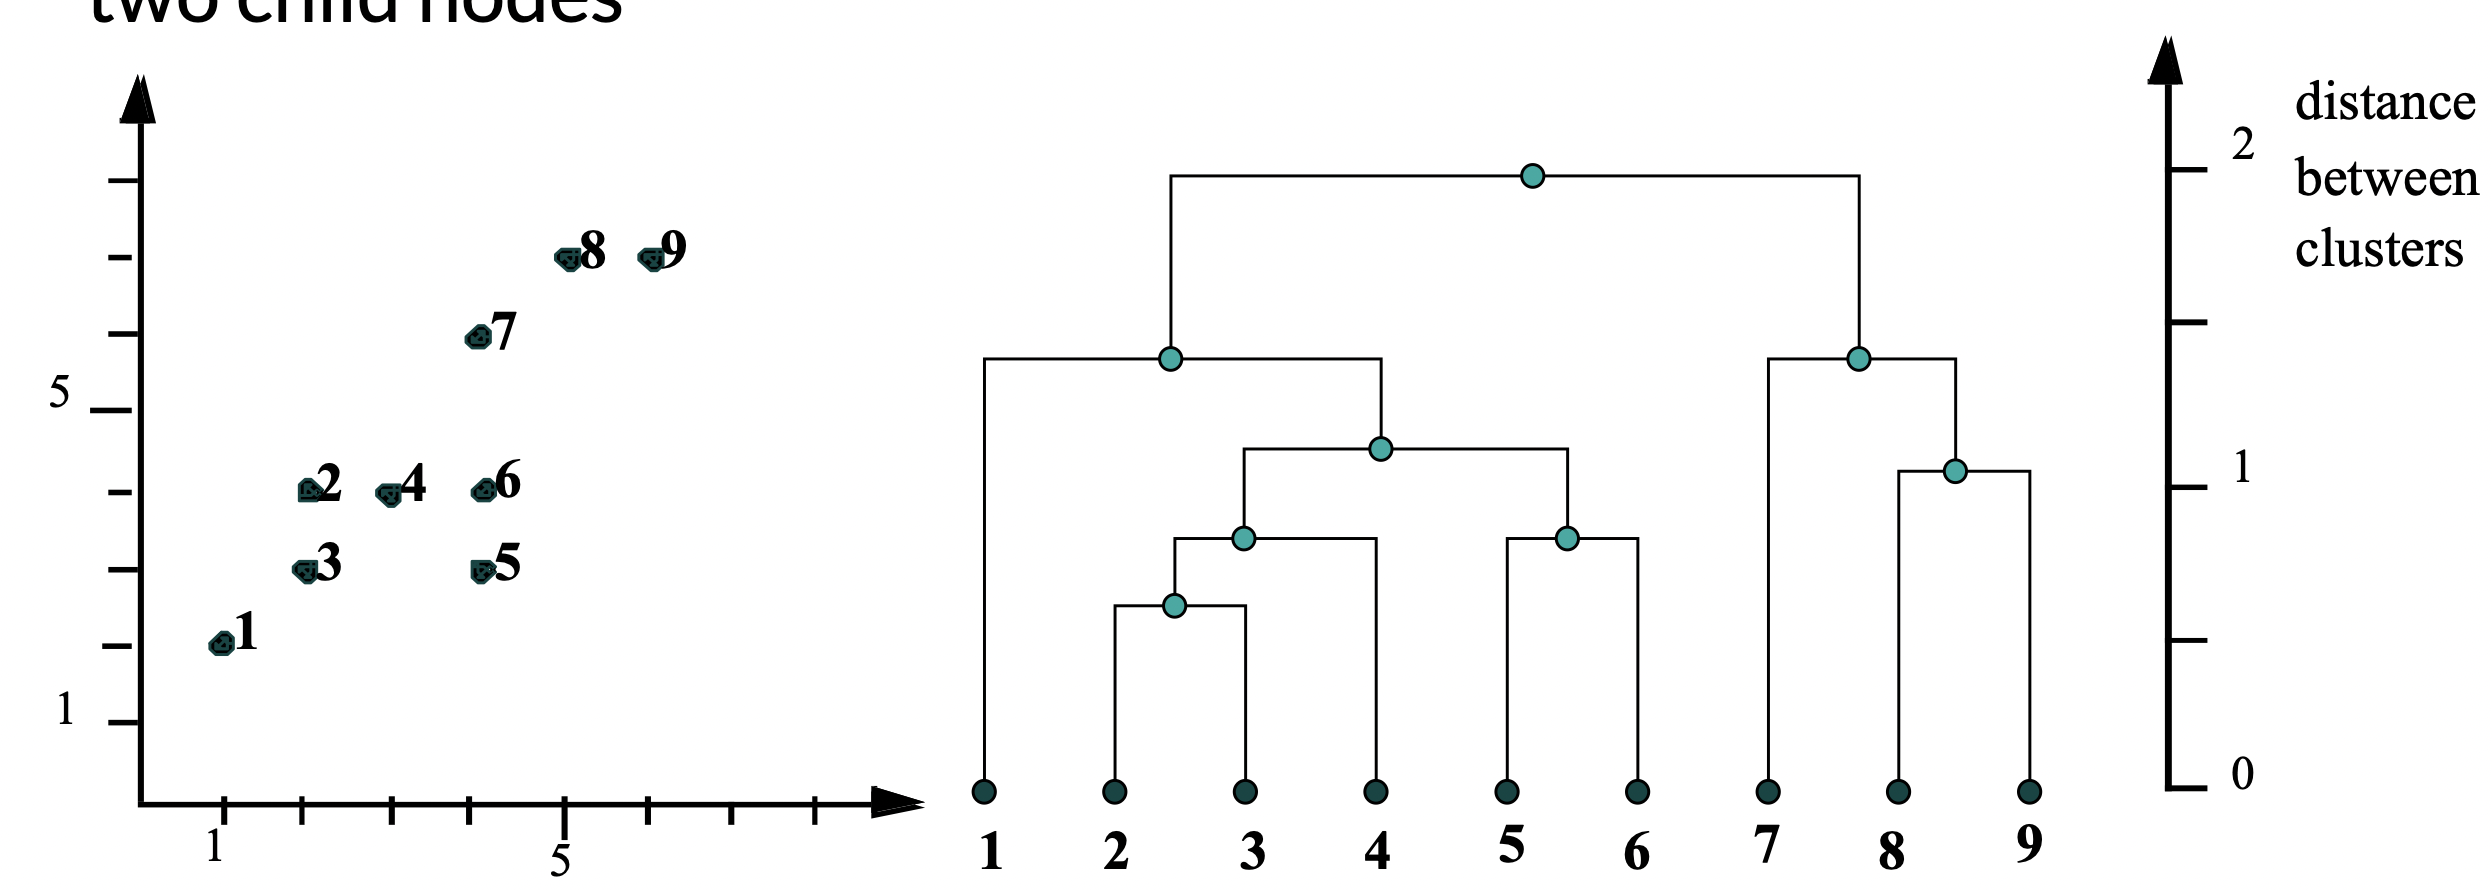
\includegraphics[width=1\textwidth]{images/dendogram.png}
\end{center}

Agglomerative hierachical clustering for a set of objects
\begin{itemize}
    \item Requires distance function
    \item Each object starts as own initial cluster
    \item Compute all pairwise distances between initial clusters, then merge closest pair
    \item Repeat
\end{itemize}

There is also the \emph{single-link} method and its variants. Following distance functions are common.
\begin{itemize}
    \item Single-link distance $dist_{sl}(C_i, C_j) = \min_{x \in C_i, y \in C_j} dist(x, y)$
    \item Complete-link $dist_{cl}(x, y) = \max_{x \in C_i, y \in C_j} dist(x, y)$
    \item Average link $dist_{al}(C_i, C_j) = \frac{1}{|C_i||C_j|} dist(x,y)$
\end{itemize}

\subsubsection{OPTICS: Ordering points to identify the clustering structure}
    We can also establish a hierarchy of density-based clusters. Dense clusters are contained in less dense clusters. The \emph{OPTICS} algorithm tries to process things in the right order in order to establish this kind of clustering. 
    
    Some basic notions are: If we find minpts, we can find object distance $\varepsilon^* \leq \varepsilon$
    
    \begin{itemize}
        \item Core-distance c-distance is the smallest distance such that $o$ is a core object (If it is less than $\varepsilon$)
        \item Reachability-distance r-dist is the smallest distance $p$ that is directly density reachable from $o$ (if it is less than $\varepsilon$)
    \end{itemize}
    
    \m{
        rdist(x,y) = \begin{cases}
            dist(x, y) & \text{if } dist(x,y) > cdistance(y) \\
            cdistance(y) & \textif{if } dist(x,y) < cdistance(y) \\
            ? & \textif{if } dist(x,y) > \varepsilon\end{cases}
        }
    
\begin{center}[h]
    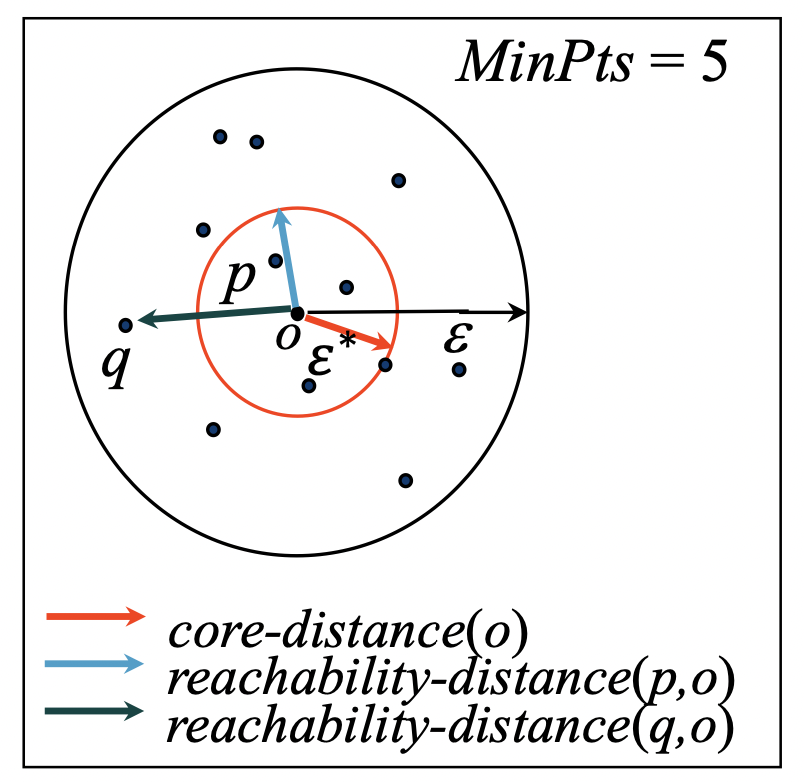
\includegraphics[width=0.4\textwidth]{images/reachability.png}
\end{center}

The basic idea behind the OPTICS algorithm is as follows:
\begin{itemize}
    \item It maintains a basic data structure (control list) that memorises the shortest reachability distance seen so far (distance of a jump to that point)
    \item It visits each point, and always makes the shortest jump
    \item It outputs the order of points, coredistances of points and reachability of points
\end{itemize}

The algorithm proceeds as follows:
\begin{enumerate}
    \item For $o$ in $D$
    \item if $o$ is not processed, insert $(o, ?)$ intro $CL$
    \item while $CL$ is non-empty \begin{enumerate}
        \item select first element $(o, rdist) \in CL$
        \item Retrieve $N_\varepsilon (o)$ and check if $cdist = coredist(o)$
        \item Set $o$ to be processed
        \item Write $(o, rdist, cdist)$ to file
        \item If $o$ is a core object at any distance $dist \leq \varepsilon$, then \begin{enumerate}
            \item Foreach $p \in N_{\varepsilon}(o)$ not yet processed, determine if $rdist_p = reachabilitydist(p, o)$, then
            \item if $(p, _)$ not in $CL$, insert $(p, rdist_p)$ into $CL$
            \item Else if $(p, old\_r\_dist) \in CL$ and $r\_dist_p < old\_r_dist$, update $(p, r_dist) \in CL$
        \end{enumerate}
    \end{enumerate}
\end{enumerate}

Finding a density based clustering w.r.t to $\varepsilon^* \leq \varepsilon$ and minpts afterwards goes as follows:
\begin{itemize}
    \item Start with $o$ with $cdist(o) \leq \varepsilon^*$ and $rdist(o) > \varepsilon^*$
    \item Continue while $rdist(o) \leq \varepsilon^*$
\end{itemize}

The running time is approx the runningtime of DBSCAN.

The reachability plot is easy to analyse. Large reachability distance equals low density, and is independent of the dimension of the data. 

\begin{center}[h]
    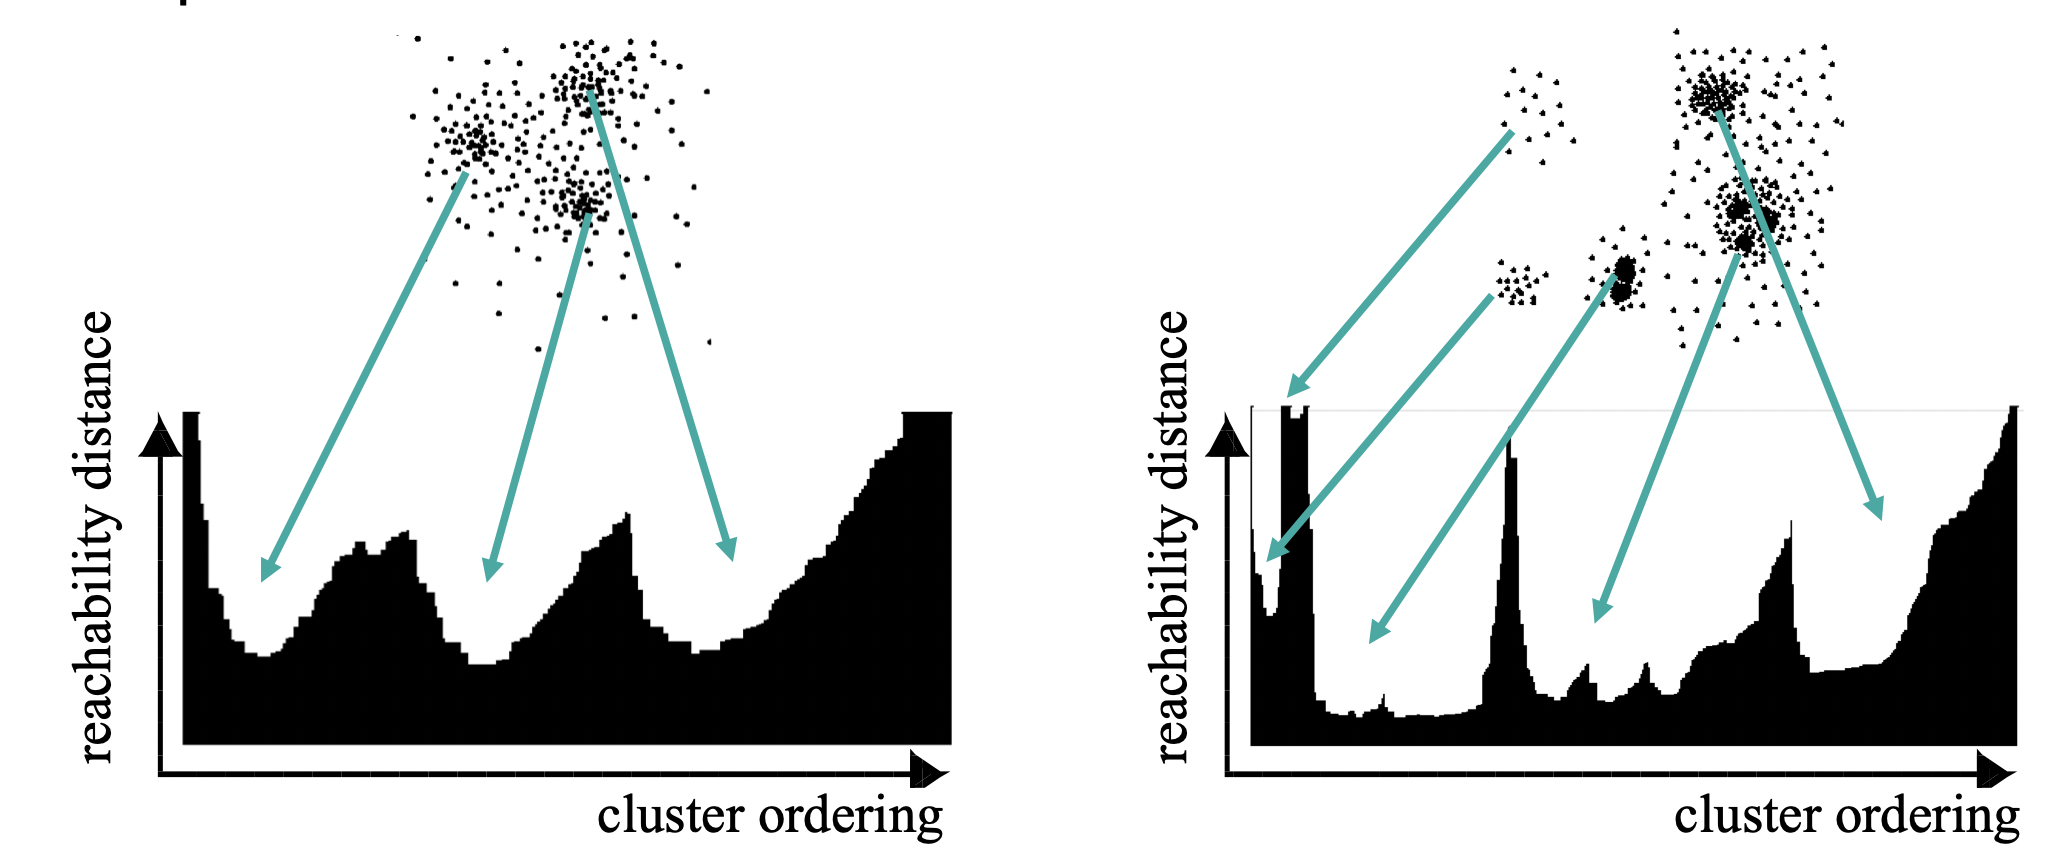
\includegraphics[width=0.4\textwidth]{images/reachabilityplot.png}
\end{center}

OPTICS is relatively insensitive to parameter settings, and results are good if the parameters are large enough.

\subsubsection{Advantages and disadvantages of hierarchical clustering with OPTICS}
The advantages are

\begin{itemize}
    \item It does not require the number of clusters to be known in advance
    \item Very roboust optics (OPTICS)
    \item Computes complete hierarchy
    \item Good visualizations
    \item A flat partition can be derived, such as cutting through the dendrogram or reachability plot
\end{itemize}

The disadvantages are
\begin{itemize}
    \item No backtracking, greedy splits and merges
    \item May not scale well. It examines many objects in order to split and merge. Runtime for standard methods is $O(n \log n)$, and for OPTICS without indexing it is $O(n^2)$
\end{itemize}

\subsubsection{BIRCH: Balanced iterative reducing and clustering using hierarchies}
With BIRCH, we are reducing the data set, then performing clustering in order to get a temporary result, and then using approximate results for full dataset. 

Specifically, the BIRCH algorithm has two stages.
\begin{itemize}
    \item Phase 1: Scan DB to build an in-memory CF (Clustering Feature) tree, which is a multi-level compression that tries to preverse inherent clustering structure
    \item Phase 2: Use an arbitrary clustering algorithm to cluster the leaf nodes of the CF tree
\end{itemize}
It scales linearly, and finds a good clustering with a single can and improves the quality with a few additional scans. It only handles numeric data, and is sensitive to order of data records.

The basic idea is as follows:
\begin{itemize}
    \item It constructs a partitioning of the data into micro-clusters using an efficient index like structure
    \item Microclusters, that is sets of objects are described in a compact way with CFs
    \item CFs are organised hierarchically in a balanced tree
    \item A standard clustering algorithm is then applied to the leaf nodes of the CF tree
\end{itemize}

\subsubsection{Clustering features}
A clustering feature $CF = (N, LS, SS)$ of a set point of points $\set{X_i}$ consists of
\begin{itemize}
    \item $N = |C|$ (Number of points in cluster)
    \item $LS = \sum_{i=1}^{N}{X_i}$ (Linear sum of the data points in C)
    \item $SS = \sum_{i=1}^{N}X_i^2$ (Square sum of the data points)
\end{itemize}
This is enough to compute centroids, measures of compactness, distance measures for clusters and so on. 

The CF additivity theorem says that CFs can be computed incrementally (Note that we only have sums, which distribute, so when we receive new data, we simply add it to the previous sums). 

\subsubsection{CF trees}
A CF tree with parameters B, L, T then consists of 
\begin{itemize}
    \item An internal node contains at most $B$ entries $[CF_i, child_i]$
    \item A leaf node contains at most $L$ entries $[CF_i]$
    \item The diameter or radius of all entries in a leaf node is at most $T$ (according to a certain distance metric)
    \item Leaf nodes are connected via prev and next pointers
\end{itemize}

The tree is constructed by
\begin{itemize}
    \item Transform point $p$ into CF vector $CF_p = (1, p, p^Tp)$
    \item Insert $p$ in the same way as in a $B+$ tree
    \item If threshold $T$ is violated by insertion, then split the leaf node and reorganize tree analog to that of $B+$ trees.
\end{itemize}

\subsubsection{The BIRCH algorithm}
    The BIRCH algorithm works as follows:
    \begin{itemize}
        \item Phase 1: Scan all data points and build in memory CF tree using given amount of memory and recycling space
        \item Phase 2: Condense into desirable length by building a smaller CF tree
        \item Phase 3: Global clustering (with any clustering algorithm) on the CF feature vectors
        \item Phase 4: (Optional) refine with more passes
    \end{itemize}
Basically, we can tweak the tree to our liking, and then cluster with it.

The advantages of the algorithm are
\begin{itemize}
    \item Compression factor can be tuned to the available memory
    \item Efficient construction of a microclustering $O(n)$
    \item Good clustering result for the partitioning iterative refine clustering algorithm algorithms such as $k$-means and $k$-medoid when applied to only the leaf nodes of a CF tree.
\end{itemize}
Disadvantages are
\begin{itemize}
    \item Only for data from a Euclidean vector space (linear sum, square sum, mean etc must be defined)
    \item Sensitive to the order of data records
    \item Entries are limited by page size
    \item Different parameters to tune
\end{itemize}

\subsection{Subspace clustering}
    Irrelevant dimensions can obscure good results. Too many dimensions also make it hard to interpret results. When we increase the number of dimensions, points are pushed further apart and dimensions become increasingly sparse. Distances converge and become meaningless. We therefore want to be able to use only relevant dimensions for different clusters. 
    
    
\subsubsection{CLIQUE}
    CLIQUE considers regions at a time. A region is considered dense if it contains more than $\tau$ points. It uses a grid based approach where each dimension is partitioned into $\chi$ intervals. A cluster is then a union of densely connected regions. 
    
    Because there are $O(2^d)$ subsets of dimensions for points in $d$ dimensions, we will use a greedy bottom-up approach. We start with an empty set of dimensions, and then iteratively include new dimensions.
    
    Density is \emph{monotonic}. If a region $r$ is dense in a $k$-dimensional space $s$, then any projection of $r$ into a $k-1$-dimensional subspace is sense (The a-priori principle). Think of points in 2d that are dense in a grid high on the y-axis, they will also be dense if projected on to the line (1d). 
    
    The CLIQUE algorithm works as follows:
    \begin{itemize}
        \item Find all dense areas in $1D$
        \item $k = 2$
        \item Repeat \begin{itemize}
            \item Generate all candidate $k$-dimensional cells from dense $k-1$-dimensional cells
            \item Eliminate cells that have fewer than $\tau$ points
            \item Increment $k$
        \end{itemize}
        \item End when there are no candidate $k$-dimensional cells
    \end{itemize}
    Find clusters by taking union of all adjacent high-density cells, then summarize each cluster by using a set of inequalities (That specify the boundaries of each cell), such as $3 \leq a_1 \land 4 \leq a_2$ etc.
    
    For each dense region, we need to check $2k$ neighbours. That gives us $2kn$ accesses to our data structure. 
    
    Furthermore, finding the maximal sets of connected dense regions is a graph problem where the search space is a graph. DFS can be used here. Basically look for components.
    
\subsubsection{Advantages and disadvantages of CLIQUE}
    The good things about CLIQUE is
    \begin{itemize}
        \item Automatic detection of subspaces with clusters
        \item Automatic detection of clusters
        \item No assumptions about the distribution of data
        \item Insensitivity to the order of the data
        \item Good scalability w.r.t to the number $n$ of data points
    \end{itemize}
    The bad things about CLIQUE are
    \begin{itemize}
        \item Accuracy of result depends on the number of partitions $\chi$
        \item We need heuristics that restrict search on all subsets of dimensions. Possibly not all subspaces with clusters are found
    \end{itemize}
    
\subsubsection{SUBCLU} 
One drawback of CLIQUE is that it depends on grid positioning. If they are not adequately oriented or shaped, clusters can be missed.

\begin{center}
    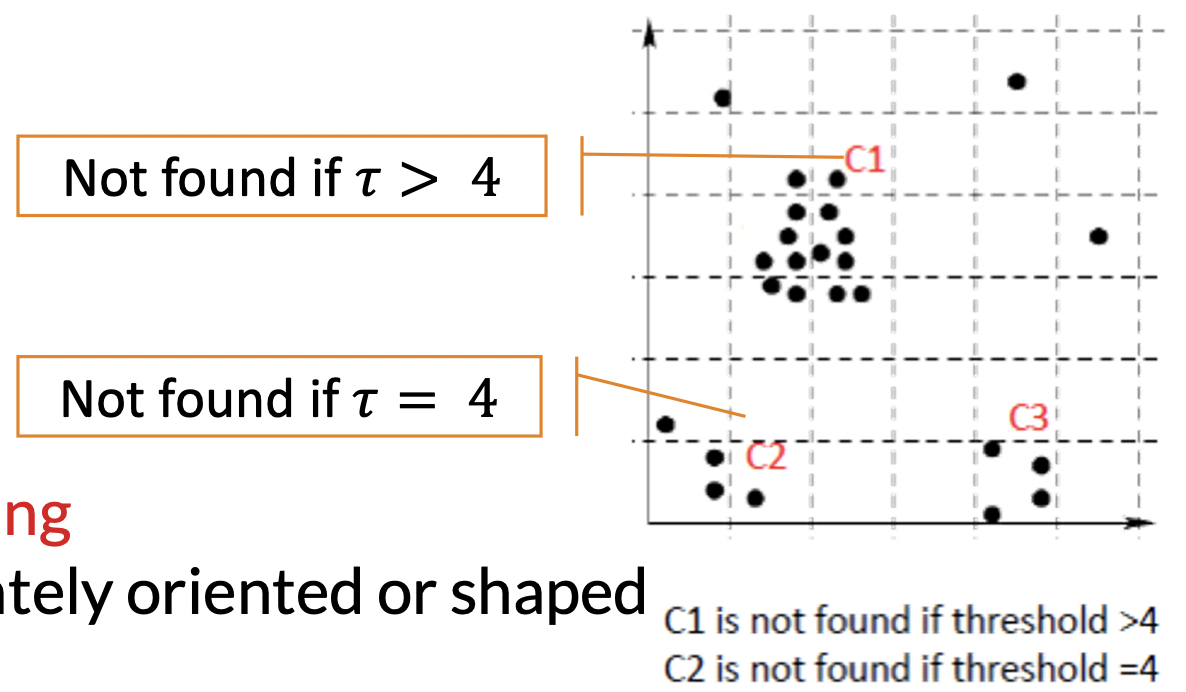
\includegraphics[width=0.5\textwidth]{images/notfound.png}
\end{center}

Here is where SUBCLU (Density-connected subspace clustering) comes into the picture. It is an extension of DBSCAN. Core-objects, density reachability and connectivity is defined for subspaces. A key property is the monotonicity of density reach-ability w.r.t dimensionality. If $p$ and $q$ are density-connected in $k$-dimensional space, all their projections in $k-1$ are also density-connected.

The algorithm is to iteratively apply DBSCAN at each step to generate $k$-dimensional clusters as in CLIQUE.

The advantages are
\begin{itemize}
    \item Automatic detection of subspaces with clusters
    \item Automatic detection of clusters
    \item No assumptions on data distributions
\end{itemize}
The disadvantages are
\begin{itemize}
    \item Parameter settings highly affect clustering results
    \item Is challenged by large differences in densities
    \item Computations is at least $O(n^2)$, typically much greater depending on dimensionality of largest subspace clsuter
\end{itemize}

\subsection{Projected clustering}
    Rather than proceeding bottom-up, we proceed top down. We start with all the dimensions, then we gradually project down to reveal clusters. 

    The goal is to identify correct projections for each object. Different from subspace clustering, each object is assigned to exactly one cluster. This avoids issues with redundancy, but we may lose some clusters (object has to be assigned to one of the available options). Some implementations allow for a nose cluster.
    
\subsubsection{PROCELUS: Projected clustering}
    The basic idea is to partition clusters in projections, based on $k$-medoid. 
    
    The steps are
    \begin{itemize}
        \item We start with an initial partition of the objects
        \item Then iteratively assign objects to a medoid. We compute the quality of our clusterings. 
        \item Sets of medoids associated with sets of dimensions (our projections)
        \item We improve both the partitions and projections iteratively
    \end{itemize}
    
    The PROCLUS algorithm has parameters $k$, which is the number of clusters (as in $k$-medoid), and $i$ which is the average number of dimensions. The algorithm proceeds in $3$ phases. 
    
    First the initialisation phase, we select a set of medoid candidates. Second, the iterative phase, we improve medoids and compute dimensions sets for each medoid. Third, the cluster refinement stage, we improve the quality of the clustering.
    
    A \emph{Projected Cluster} is a set of objects $C$ and a set of dimensions $D$, such that the objects in $C$ are closely clustered in the subspace defined $D$. 
    
    The concept of \emph{Closely clustered} requires that we compare objects in different subspaces. We normalize with respect to dimensionality. PROCLUS uses the Manhatten segmential distance $d(x, y) = \frac{1}{|D|}\sum_{i \in D}{|x_i - y_i|}$. 
    
    The initialisation phase goes as follows: 
    \begin{itemize}
        \item Pick a sample of representative data points
        \item They should stretch across the sample
        \item The set should be a superset of the set of medoids
        \item Medoids are chosen from representative points
    \end{itemize}
    In practice, we will use a greedy algorithm and select $A \cdot k$ points that are well-seperated. 
    
    The iterative phase goes as follows:
    \begin{itemize}
        \item Choose random set of $k$-medoids from representative points
        \item Determine optimal set of dimensions for each medoid
        \item Assign all objects to the nearest medoid
        \item Choose current clustering if it is better than the previous until termination
    \end{itemize}
    Replace bad medoids with random medoids. The termination criterion is when clustering does not change within a certain number of iterations.
    
   We need to be able to find the optimal dimensions for each medoid. We will measure $z_{ij}$ for each cluster $i$ and each dimensional $j$ to evaluate that dimension relative to all dimensions in all clusters. It should reflect the spread in that cluster in that dimension relative to all dimensions. 
   
   For each medoid $m_i$, we will calculate the average distance $X_{ij}$ of objects in $L_i$ to $m_i$ in dimension $j$. $L_i$ is the hypersphere with radius of distance to the nearest medoid. We will then average the distance over all dimensions. 
   \m{
    Y_i = \frac{1}{d}\sum_{j=1}^{d}X_{ij}
   }
   Each dimension $j$ in cluster $i$ is evaluated iteratively to other dimensions of cluster. If $X_{ij} - Y_{i} < 0$ then objects in cluster $i$ are more correlated than the average in dimension $j$. 
   
   In order to compare these values to that of other clusters, we will normalize $(X_{ij} - Y_{ij})$ by standard deviation in cluster $i$. 
   \m{
    Z_{ij} = \frac{1}{\sigma_i}(X_{ij} - Y_{i})
   }
   Where \m{
    \sigma_i = \sqrt{
    \frac{1}{d-1} \sum_{j=1}^{d}{(X_{ij} - {Y_i})^2}
    }
   }
   Small values indicate the best dimensions, and high correlation means clusterings exist in those dimensions. Assign globally the best dimensions to their clusters, but at least two per cluster. This is the dimension set for each medoid. Remember to assign objects to their nearest Medoid using manhatten distance.
   
   The iterative phase is now 
   \begin{enumerate}
       \item Calculate all $Z_{ij}$ values. There are $kd$ of these. Sort them.
       \item Pick the best two values for each cluster, to assure that there are at least two dimensions for each cluster.
       \item Greedily pick best $k(l-2)$ remaining values
       \item If $Z_{ij}$ is picked, then add dimension $j$ to $D_i$
       \item Return sets $D_k$ for each medoid
       \end{enumerate}
       
     In the update phase, we now look at the centroid as basis for cluster spread analysis. Measure the average distance of object to its centroid per dimension. Low values mean objects in each cluster are close
     \m{
        \frac{1}{N} \sum_{i=1}^{l} |C_i| w_i
     }
     Where $W_i$ is average distance of object in cluster $C_i$ to its centroid per dimension $j$ that is part of the dimension set $D_i$ of that cluster
     \m{
        w_i = \frac{1}{|D_i|}\sum_{j \in D_i}{V_{ij}}
     }
     Where $V$ is the average distance of objects in $C_i$ to centroid $C_i$ in dimension $j$.
     
     Now we replace bad medoids. They are bad if their clusters $C_i$ is the smallest (least number of objects), or $C_i < \frac{N}{k} \cdot mindeviation$ where mindeviation is a constant (in experiments 0.1). Maybe it is an outlier or member in a cluster of another medoid. 
     
     Finally, in the refine phase, we determine the optimal dimension for each medoid, which is the same procedure as in the iterative phase, but $L_i = C_i$. Reassign all objects to cluster $C_i$ whose medoid is closest (relative to the new sets of dimensions $D_i$.
     
     An object is an outlier if its segmental distance to each medoid exceeds the radius of the medoids sphere of influence.
     
\subsubsection{Advantages and disadvantages of PROCELUS}
    Advantages are
    \begin{itemize}
        \item Based on full high-dimensional space
        \item Simpel but efficient projected clustering
    \end{itemize}
    Disadvantages are
    \begin{itemize}
        \item Relies on cluster-based locality assumption: subspace of each cluster is learned from local neighborhood of its medoid
        \item Forces projected clusters to have convex shape
        \item Medoids are chosen only from initial sample set
        \item Heighly heuristic and is sensitive a large number of input parameters ($k, l, A, mindeviation$)
    \end{itemize}